\documentclass[11pt]{article}
\usepackage[T1]{fontenc}
\usepackage[margin=1in]{geometry}
\usepackage{amsmath,amssymb}
\usepackage{graphicx}
\usepackage{microtype}
\usepackage{xcolor}
\usepackage[colorlinks=true,linkcolor=blue!55!black,urlcolor=blue!65!black]{hyperref}

\title{Question 6.7 on Quasi-Local Operators\\
Was Answered by Ozawa}
\author{Literature-resolution packet for arXiv:1809.00532}
\date{27 August 2026}

\begin{document}
\maketitle

\begin{center}
\fbox{\begin{minipage}{0.91\textwidth}
\textbf{Status: literature already answered.}
Ozawa proves that every uniformly locally finite metric space containing a
sequence of expanders has a quasi-local operator on $\ell^2(X)$ that is not
approximable by finite-propagation operators. This is exactly the example
requested in Question 6.7 of Špakula--Zhang.
\end{minipage}}
\end{center}

\section{The source question}

Špakula and Zhang \cite{SZ} prove equality of the uniform Roe and quasi-local
algebras under Property A and ask on PDF page 20:

\begin{quote}
\textbf{Question 6.7.} Is there an example of a space $X$ with bounded
geometry and a quasi-local operator on (say) $\mathcal B(\ell^2(X))$ which
does not belong to the uniform Roe algebra $C_u^*(X)$?
\end{quote}

Here $C_u^*(X)$ is the norm closure of the finite-propagation operators, while
$C_{ql}^*(X)$ is the algebra of quasi-local operators. Thus the question asks
whether $C_u^*(X)\subsetneq C_{ql}^*(X)$ can occur.

\begin{center}
  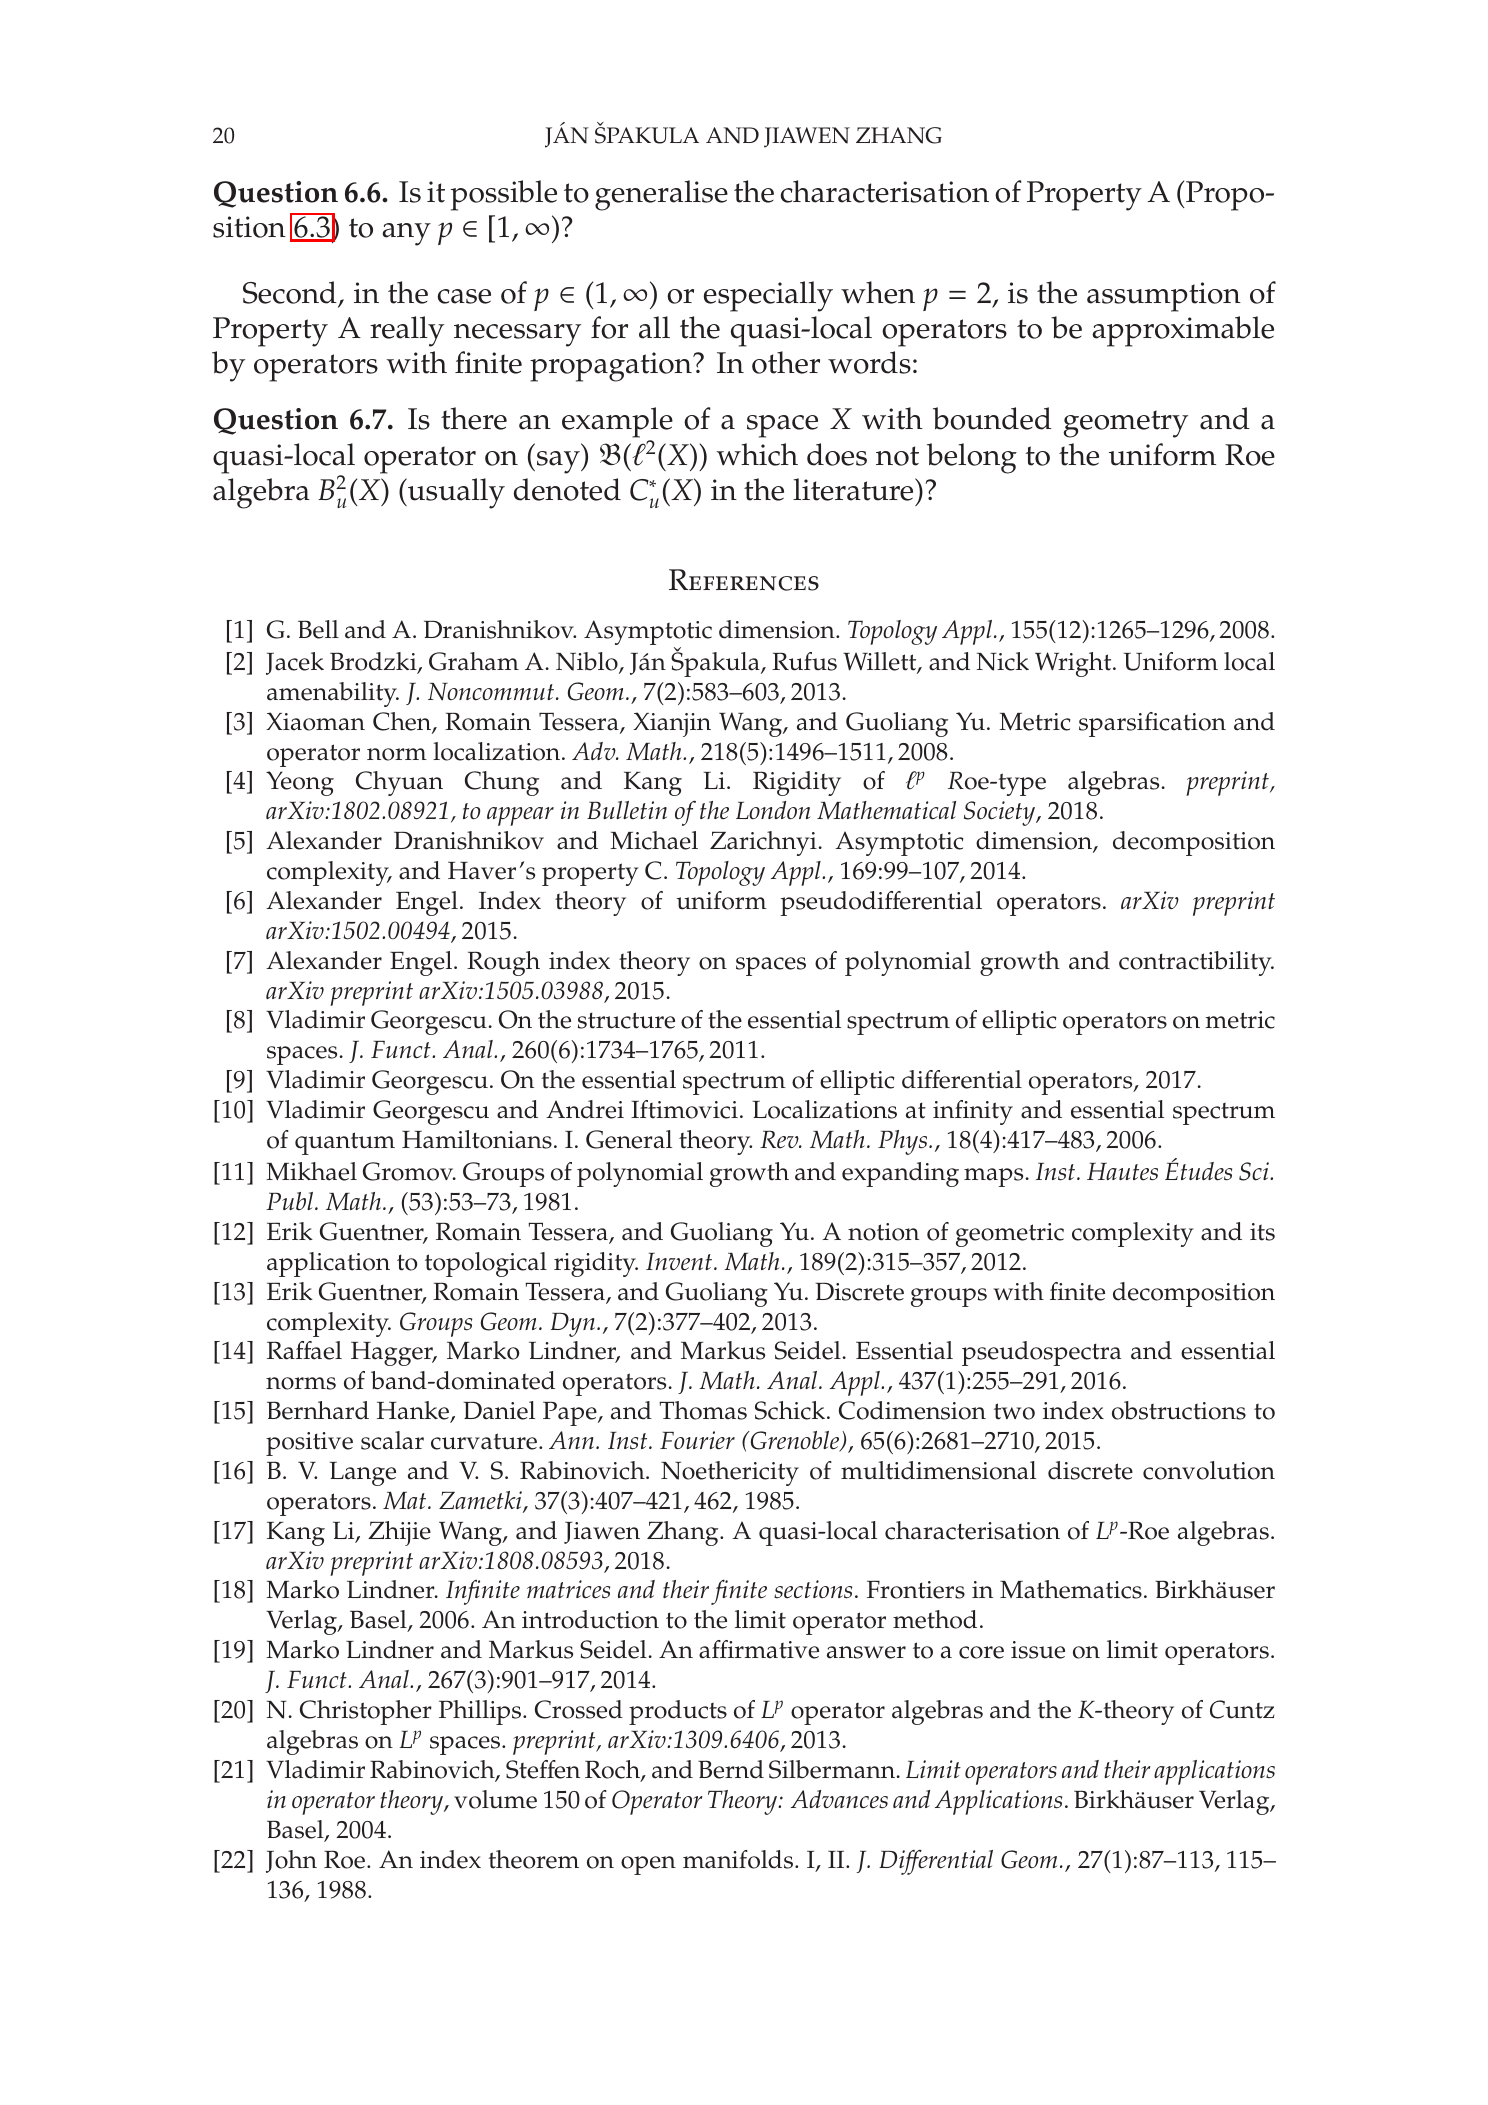
\includegraphics[width=\textwidth,height=0.67\textheight,keepaspectratio]
    {figures/source_question_page20.png}
\end{center}

\clearpage
\section{Ozawa's exact answer}

Ozawa's paper \cite{O} studies the same two algebras on uniformly locally
finite (equivalently, bounded-geometry in this setting) metric spaces. Its
abstract says that the results yield a quasi-local operator not approximable
by finite-propagation operators. The introduction proves:

\begin{quote}
\textbf{Theorem A.} The $C^*$-algebra $\prod_n M_n$ does not embed into the
uniform Roe algebra $C_u^*[X]$ of any uniformly locally finite metric space
$X$.

\textbf{Theorem B.} The $C^*$-algebra $\prod_n M_n$ embeds into the
quasi-local algebra $C_{ql}^*[X]$ of a uniformly locally finite metric space
$X$, provided that $X$ contains a sequence of expanders.

\textbf{Corollary C.} For every uniformly locally finite metric space $X$
containing a sequence of expanders, the inclusion
$C_u^*[X]\subset C_{ql}^*[X]$ is proper. Equivalently, there is a quasi-local
operator which is not approximable by finite-propagation operators.
\end{quote}

Choosing any bounded-geometry coarse disjoint union of finite expanders gives
the requested $X$. Properness produces an element
$T\in C_{ql}^*(X)\setminus C_u^*(X)$, which is precisely the requested
operator. There is no mismatch in category or closure: both papers work on
$\ell^2(X)$ and define the uniform Roe algebra as the norm closure of
finite-propagation operators.

The connection is explicit rather than inferred only from terminology.
Ozawa cites Špakula--Zhang as [SZ], states that they prove equality for
Property A spaces, and cites page 20 of the earlier literature when framing
the equality problem.

\begin{center}
  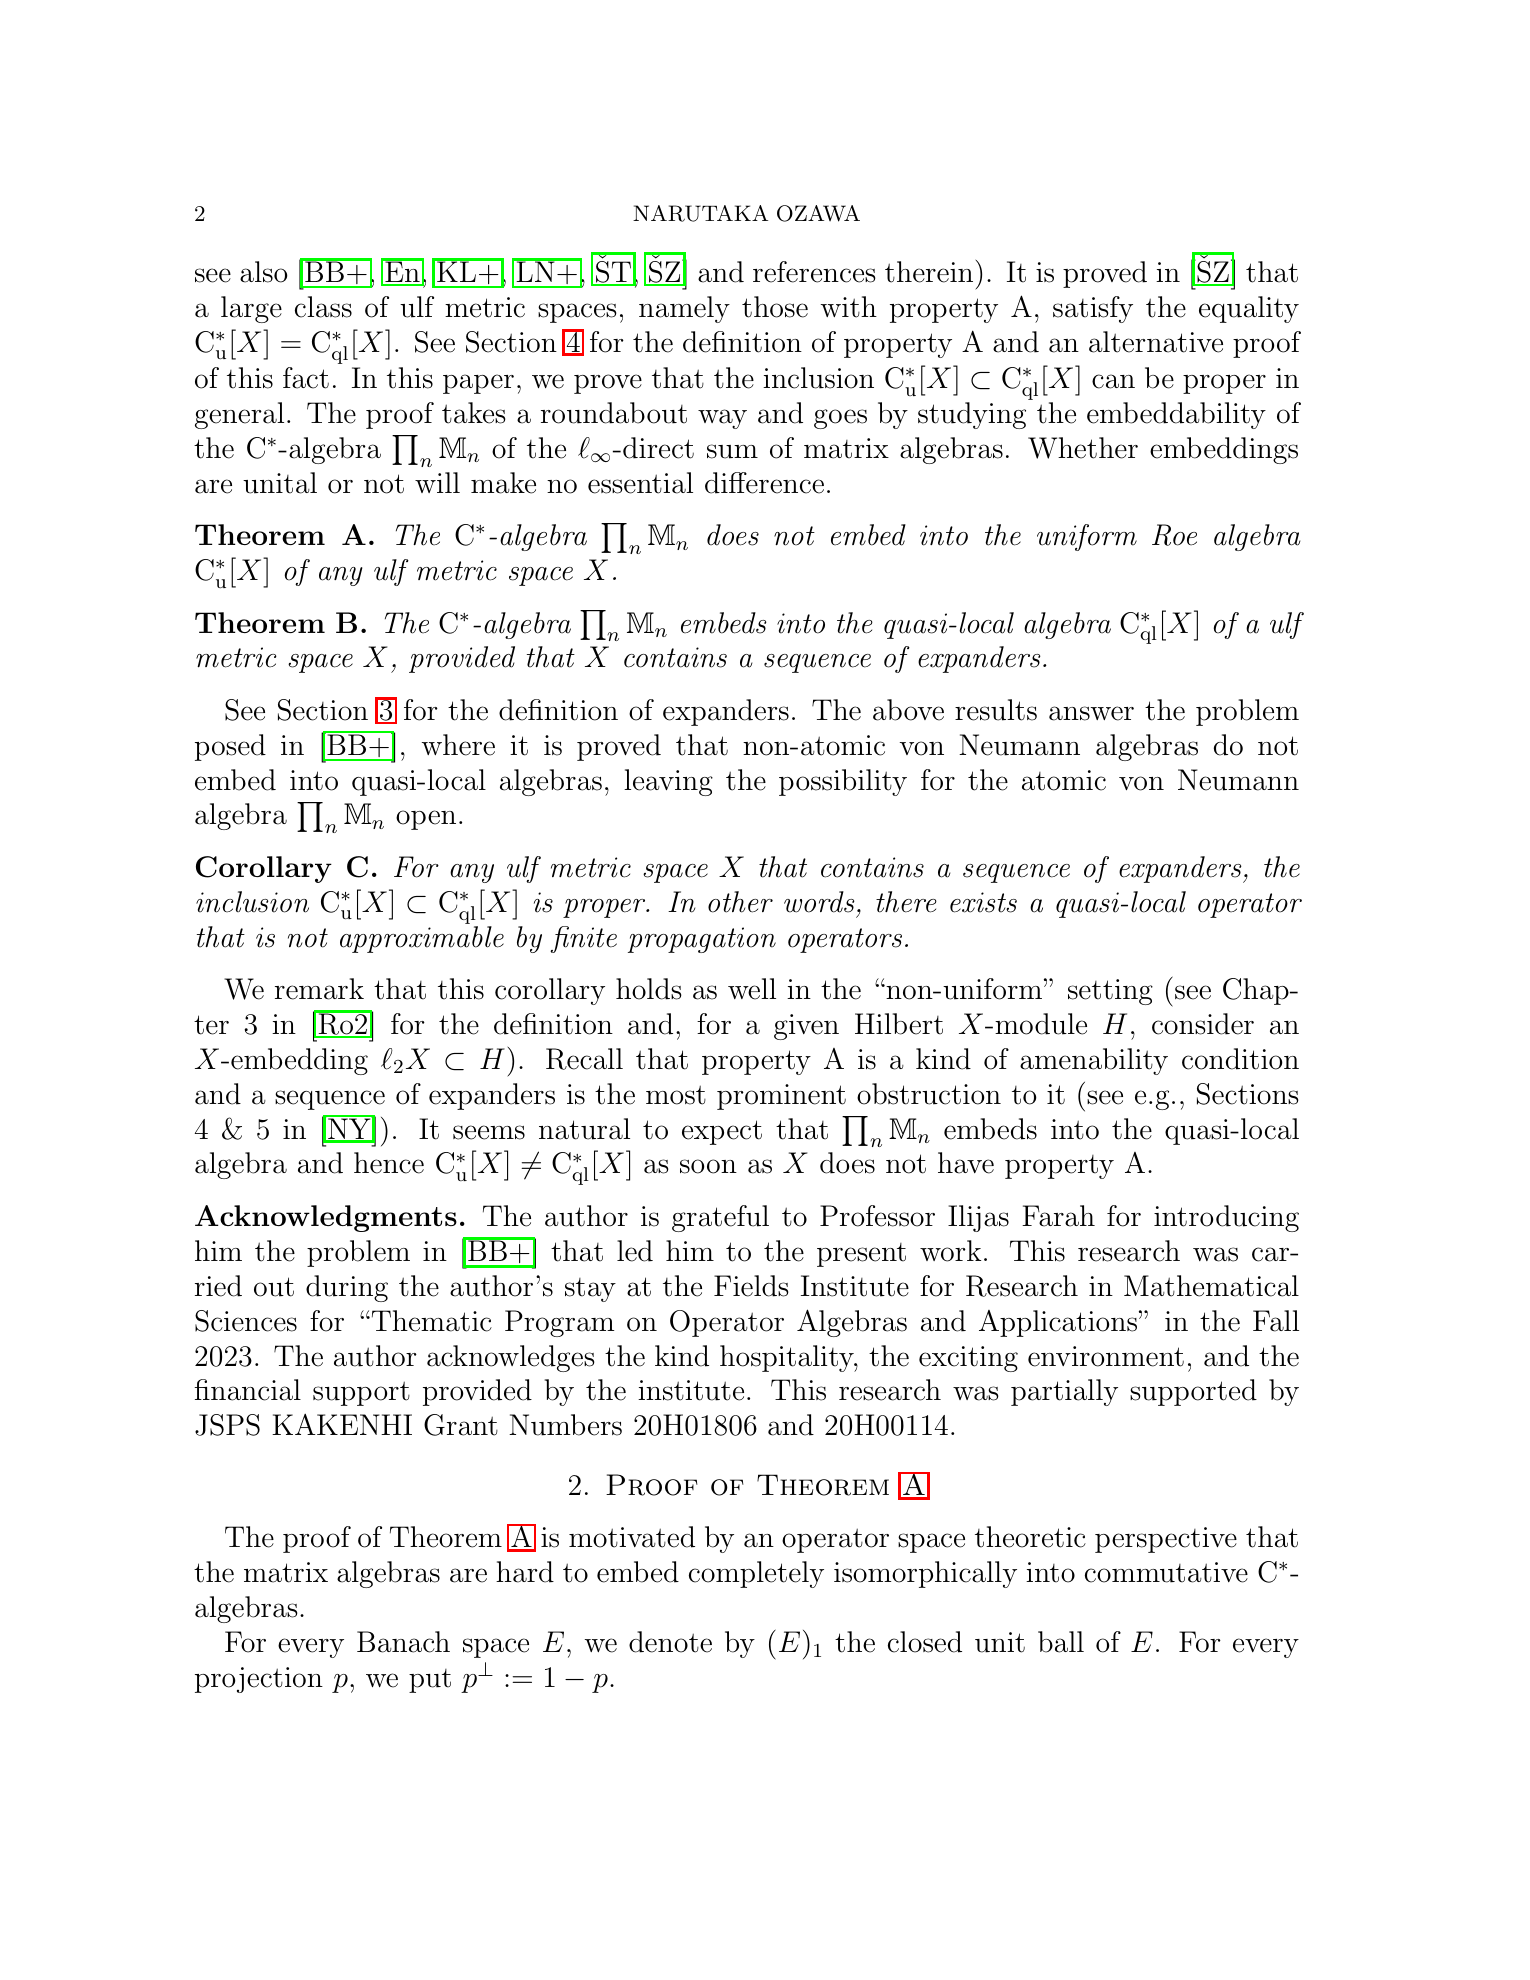
\includegraphics[width=\textwidth,height=0.68\textheight,keepaspectratio]
    {figures/answer_theorems_page2.png}
\end{center}

\clearpage
\section{Audit and scope}

The theorem match is exact:
\begin{itemize}
\item bounded geometry corresponds to Ozawa's uniformly locally finite
hypothesis;
\item containing a sequence of expanders supplies explicit eligible spaces;
\item proper inclusion supplies a quasi-local operator outside the uniform
Roe algebra;
\item being outside $C_u^*(X)$ means not being norm-approximable by
finite-propagation operators.
\end{itemize}

Therefore Question 6.7 has a complete affirmative literature answer. No new
proof or counterexample should be promoted for that question. Ozawa's result
does not answer the distinct $p$-generalization asked in Question 6.6.

\paragraph{Search audit.}
The run's cheap indexes contained no prior packet for arXiv:1809.00532. A
bounded exact-title and keyword search for quasi-local operators outside
uniform Roe algebras located arXiv:2310.03677. Its abstract, Theorems A--B,
Corollary C, and citations to Špakula--Zhang were checked against the official
arXiv PDF.

\paragraph{Human review.}
Confirm the terminology identification ``uniformly locally finite'' with the
source's bounded-geometry convention and the literal statement of Corollary
C. The substantive match is otherwise direct.

\section*{Answer-paper abstract page}
\begin{center}
  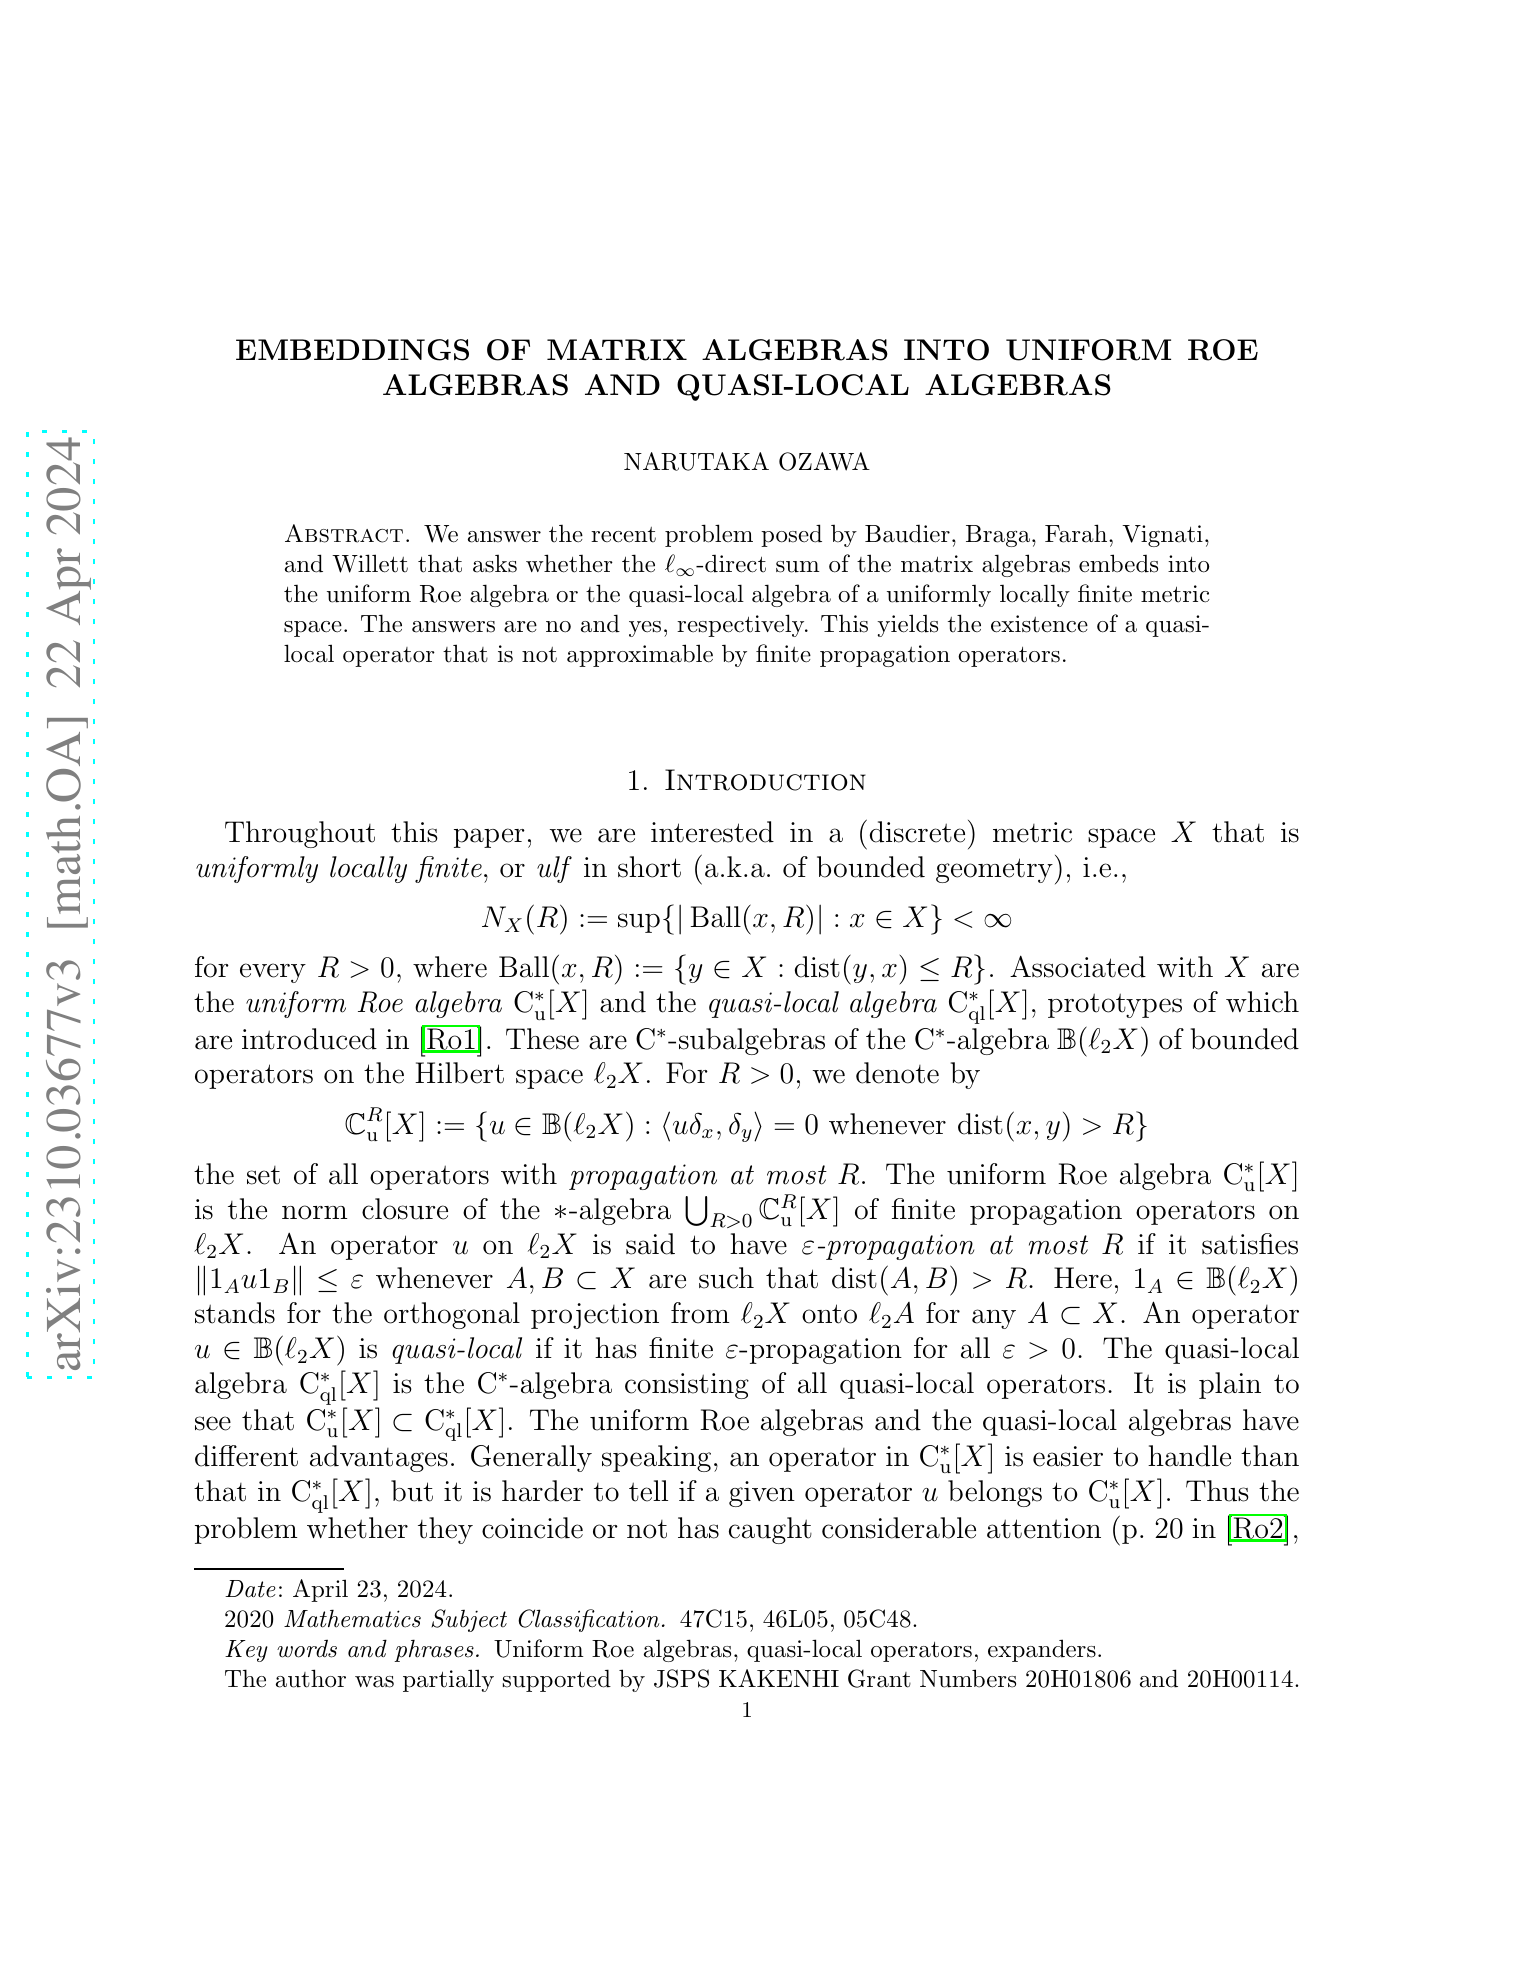
\includegraphics[width=\textwidth,height=0.76\textheight,keepaspectratio]
    {figures/answer_abstract_page1.png}
\end{center}

\begin{thebibliography}{9}
\bibitem{SZ}
J.~Špakula and J.~Zhang,
\emph{Quasi-Locality and Property A},
J. Funct. Anal. 278 (2020), 108299; arXiv:1809.00532.

\bibitem{O}
N.~Ozawa,
\emph{Embeddings of matrix algebras into uniform Roe algebras and
quasi-local algebras}, arXiv:2310.03677 (version dated 23 April 2024).
\end{thebibliography}

\end{document}
